\chapter{Metodología}
\label{chap:metodologia}

\drop{E}n este capítulo se van a exponer brevemente las características principales de las metodologías elegidas para el desarrollo de este \acs{TFG}. En este caso se ha decidido escoger Scrum, una metodología ágil para la gestión de proyectos y, en cuanto a la metodología de desarrollo de software, se ha escogido el ciclo de vida iterativo e incremental.

\section{Metodología de Gestión de Proyectos: Scrum}
Scrum \cite{Schwaber2017} es un marco de trabajo que se usa para la gestión del desarrollo de productos dentro del que se pueden emplear diferentes procesos y técnicas. Posee equipos autogestionados con sus roles, eventos, artefactos y reglas asociadas. Esta metodología se basa en dividir el proyecto en diferentes fases, de manera que una fase no puede comenzar mientras la anterior no haya terminado. Dos de los términos más importantes en Scrum son el Sprint y la Pila de Producto (\textit{Product Backlog}). El primero es un bloque de tiempo donde se crea un entregable del producto, mientras que el segundo es el conjunto de todo lo que podría ser necesario en el producto.

\subsection{Teoría de Scrum}
Scrum se basa en la teoría de control de procesos empírica, lo que asegura que el conocimiento procede de la experiencia de la toma de decisiones basadas en lo que ya se conoce, empleando un enfoque iterativo e incremental. Sus tres pilares fundamentales son \cite{Schwaber2017}:

\begin{itemize}
	\item \textbf{Transparencia}. Los aspectos significativos del proceso han de ser visibles para los responsables del resultado.
	\item \textbf{Inspección}. Los usuarios de Scrum deben inspeccionar con frecuencia los artefactos y el progreso para detectar variaciones indeseadas. Estas inspecciones no deben interferir en el trabajo.
	\item \textbf{Adaptación}. Si un inspector determina que uno o más aspectos de un proceso se desvían de ciertos límites y que el resultado será inaceptable, se procederá a un reajuste que deberá realizarse tan pronto como sea posible para evitar una posible desviación.
\end{itemize}

\newpage

\subsection{El equipo de Scrum}
Cada equipo de Scrum \cite{Schwaber2017} se compone del \textbf{Dueño del Producto} (\textit{Product Owner}), el \textbf{Equipo de Desarrollo} (\textit{Development Team}) y un \textbf{Maestro de Scrum} (\textit{Scrum Master}). Además, los equipos son autoorganizados y multifuncionales.

\subsection*{Dueño del Producto (\textit{Product Owner})}
Es el responsable de maximizar el valor del producto desde el punto de vista del negocio, puesto que es el intermediario entre el cliente y el equipo. Es decir, el Dueño del Producto es el representante del cliente. Además, posee la responsabilidad de controlar la Pila de Producto, control que se realiza mediante diferentes tareas como la de fijar sus ítems, ordenarlos, optimizar el valor del trabajo del equipo de desarrollo o asegurar que cada ítem se encuentra correctamente descrito.

\subsection*{Equipo de Desarrollo (\textit{Development Team})}
Este equipo está formado por profesionales que entregan un incremento del producto terminado que se puede poner en producción al final de cada Sprint. El equipo de desarrollo tiene las siguientes características:

\begin{itemize}
	\item \textbf{Son autoorganizados}. Nadie indica al equipo cómo convertir la Pila de Producto en incrementos.
	\item \textbf{Son multifuncionales}. Cuentan con las habilidades necesarias para crear un incremento.
	\item \textbf{No se reconocen títulos individuales}. El grupo es más importante que el individuo, es decir, el peso del trabajo que se realiza recae en todo el equipo.
	\item \textbf{No se reconocen subequipos}. Puede considerarse una derivación del punto anterior.
	\item \textbf{Cada miembro debe tener habilidades especializadas y áreas en las que enfocarse.} A pesar de esto, la responsabilidad siempre recaerá en el equipo como conjunto.
\end{itemize}

\subsection*{Maestro de Scrum (\textit{Scrum Master})}
El \textit{Scrum Master} \cite{Gomez2017} es el responsable de que Scrum se entienda y se adopte y de que el equipo sea productivo. Principalmente, es un <<facilitador>>. Trabaja muy cerca del dueño del producto y del equipo, protegiéndolo de interferencias externas, eliminando impedimentos y procurando que fluya la comunicación y la colaboración.

\clearpage

\subsection{Eventos de Scrum}
Existen eventos \cite{Schwaber2017} predefinidos cuyo fin es crear regularidad en el trabajo y minimizar la necesidad de realizar reuniones no definidas. Cada evento es un bloque de tiempo al que se le asocia una duración máxima.

\subsubsection{El Sprint}
Es un bloque de tiempo cuya duración es, como máximo, de un mes donde se crea un incremento del producto. Un nuevo Sprint comienza inmediatamente después de la conclusión del anterior y una de sus principales características es que, en cada uno, se solapan todas las etapas de la creación de un producto. Es decir, en cada iteración se realiza la planificación, análisis, creación y comprobación del entregable. El Sprint se divide en una serie de etapas, que son la \textbf{Planificación del Sprint} (\textit{Sprint Planning}), el \textbf{Scrum Diario} (\textit{Daily Scrum}) el \textbf{Trabajo de Desarrollo} (\textit{Development Work}), la \textbf{Revisión del Sprint} (\textit{Sprint Review}) y la \textbf{Retrospectiva del Sprint} (\textit{Sprint Retrospective}).

\subsubsection{Planificación del Sprint (\textit{Sprint Planning})}
Esta tarea se realiza al comienzo de cada Sprint y su finalidad es la de programar el trabajo que se realizará durante el mismo \cite{Gomez2017}. Antes, el dueño del producto revisa que la Pila de Producto se corresponde con las historias de usuario que le gustaría ver incluidas en la siguiente iteración, junto con su correcta descripción y priorización. La reunión debe terminar con unos objetivos completados: una lista de historias o \textit{Sprint Backlog} (conjunto de historias de usuario y tareas en las que se dividen), un propósito para el Sprint que sugiere el dueño del producto, el compromiso del equipo de realizar las historias, la estimación del equipo del esfuerzo necesario para realizar cada historia y, finalmente,  que todos entiendan el contenido y el alcance de todas las historias.

\subsubsection{Scrum Diario (\textit{Daily Meeting})}
El Scrum diario \cite{Schwaber2017} es una reunión de corta duración para la sincronización de las actividades y la creación del plan de actividades por parte del equipo de desarrollo.

\subsubsection{Revisión del Sprint (\textit{Sprint Review})}
Esta tarea se realiza al final de cada Sprint para inspeccionar el incremento y adaptar la Pila de Producto si fuera necesario. Se trata de una reunión informal en la que participan el equipo Scrum y los interesados.

\subsubsection{Retrospectiva del Sprint (\textit{Sprint Retrospective})}
Aquí el equipo Scrum se inspecciona a sí mismo para crear un plan de mejoras para el siguiente Sprint. Se realiza después de la revisión y antes de la siguiente planificación.

\newpage

\subsection{Artefactos de Scrum}
Los artefactos representan trabajo o valor en diversas formas que son útiles para proporcionar transparencia y oportunidades de adaptación e inspección y deben  estar al alcance de todos los participantes en el proyecto.

\subsubsection{Pila de Producto (\textit{Product Backlog})}
El \textit{Product Backlog} es uno de los elementos fundamentales, siendo una lista de todo lo que podría ser necesario en el producto. Contiene las características, funcionalidades, requisitos, mejoras y correcciones que conforman cambios a realizar sobre el producto para entregas futuras. Su responsable es el dueño del producto, incluyendo su contenido, disponibilidad y ordenación. Esta lista va evolucionando a medida que el producto y el entorno en el que se usará también lo hacen. Esto quiere decir que es dinámica, cambiando constantemente.

\subsubsection{Pila de Sprint (\textit{Sprint Backlog})}
Esta lista \cite{Gomez2017} contiene los trabajos a realizar en un Sprint determinado. Contiene las historias de usuario y las tareas identificadas por parte del equipo de desarrollo, que es quien gestiona esta lista. Al igual que la lista de producto, es dinámica y se va modificando durante el Sprint según se trabaja en lo planeado.

\subsubsection{Incremento}
El Incremento \cite{Schwaber2017} es la suma de todos los elementos de la lista de producto completados durante un Sprint y el valor de los Sprints anteriores.

\subsubsection{Gráficos \textit{burn-down} y \textit{burn-up}}
Otros artefactos importantes son las gráficas. Principalmente se usa la gráfica \textit{burn-down}, que  consiste en representar el trabajo mediante dos ejes: el vertical representa una escala numérica del trabajo (historias de usuario o <<puntos de historia>>) y el horizontal representa el tiempo. Además, se tiene una línea recta de la evolución ideal del trabajo y cada día se va comparando con lo que se ha realizado realmente para llegar finalmente a cero, lo que significaría que el trabajo se ha completado totalmente. Un ejemplo visual se encuentra en la Figura \ref{fig:burndown}, donde también se puede observar la línea \textit{velocity}, que representa la cantidad de trabajo terminado en cada iteración mediante <<puntos de historia>>. Por otra parte, los gráficos \textit{burn-up} muestran el trabajo realizado de manera creciente.

\begin{figure}[!h]
	\begin{center}
		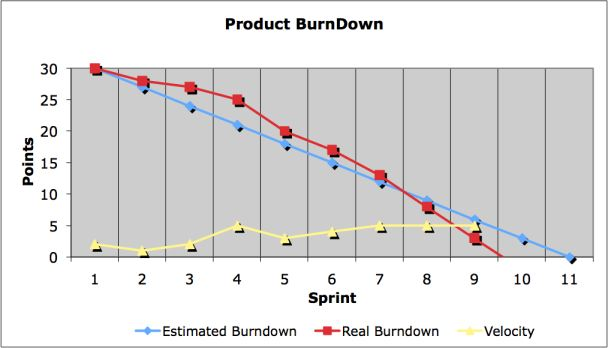
\includegraphics[width=0.7\textwidth]{/burndown_chart}
		\caption{Gráfico \textit{Burn-down}}
		\label{fig:burndown}{\url{https://www.scrum-institute.org/Burndown_Chart.php}}
	\end{center}
\end{figure}

\newpage

Así como la metodología de gestión de proyectos elegida ha sido Scrum, en cuanto al desarrollo del software se ha elegido el ciclo de vida iterativo e incremental.

%TODO: Referencia a Ismael Caballero?
\section{Metodología de Desarrollo de Software: Iterativo e Incremental}
Este ciclo de vida consiste en desarrollar por partes el producto, integrándolas progresivamente conforme se van completando, agregando más funcionalidad al sistema final. Por otra parte, en cada iteración se revisa y mejora el producto, añadiendo nuevos requisitos o mejorando los ya existentes, repitiendo un proceso de trabajo similar \cite{proyectosagiles.org}. En cierto modo, se crean <<miniproyectos>> entre los que se reparte el trabajo y cada uno representa una iteración que generará un incremento como resultado. Cada uno de estos <<miniproyectos>> sigue el esquema análisis-diseño-pruebas. Si la iteración finalmente cubre los requisitos elegidos, la siguiente puede comenzar, de otro modo los requisitos han de ser revisados. Esta metodología tiene una serie de ventajas: el riesgo del proyecto se reduce a un incremento, se previene de lanzar software incompleto o de baja calidad, hace que el esfuerzo de los desarrolladores se concentre y sea más eficiente en cada iteración y se puede conseguir una mejor colección de requisitos.

\clearpage

\section{Recursos}
Para el desarrollo de este trabajo no se requiere de hardware especial puesto que se utilizan herramientas y equipos que están disponibles para cualquier usuario doméstico. El software, por su parte, resulta más específico para el desarrollo de este trabajo ya que requiere de ciertos conocimientos más técnicos.

\subsection{Recursos Hardware}
Principalmente se va a usar un ordenador que ejecuta el sistema operativo Windows (Figura \ref{fig:winver}) para llevar a cabo la consecución del proyecto.

\begin{itemize}
	\item \textbf{Marca y modelo:} Sony VAIO F-Series.
	\item \textbf{Procesador:} Intel\textregistered{ } Core\texttrademark{ } i7-720QM @ 1.6 \acf{GHz}.
	\item \textbf{RAM:} 8 \acs{GB}.
	\item \textbf{Tarjeta Gráfica:} NVIDIA GeForce GT 330m.
	\item \textbf{Disco Duro:} 500 \acs{GB}.
\end{itemize}

\begin{figure}[!h]
	\begin{center}
		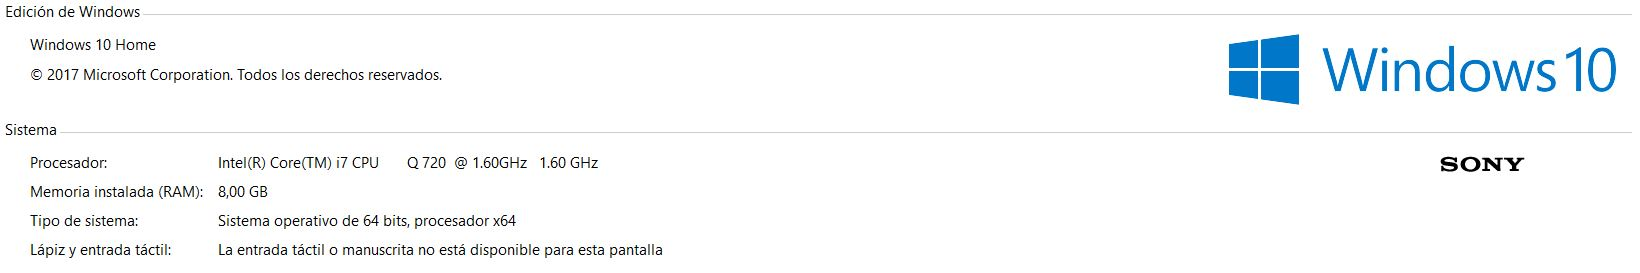
\includegraphics[width=1\textwidth]{/windows_ver}
		\caption{Información de Windows}
		\label{fig:winver}
	\end{center}
\end{figure}

Del mismo modo, se ha usado un \textit{smartphone} para comprobar el correcto funcionamiento de la aplicación.

\begin{itemize}
	\item \textbf{Marca y modelo:} LG Optimus L5 II.
	\item \textbf{Procesador:} MediaTek MT6575 @ 1 \acs{GHz}.
	\item \textbf{Sistema Operativo:} Android 4.1.2 \textit{Jelly Bean}.
	\item \textbf{RAM:} 1 \acs{GB}.
	\item \textbf{Memoria interna:} 4 \acs{GB}.
\end{itemize}

\clearpage

\subsection{Recursos Software}
Puesto que se pretende que la aplicación posea una parte de administración web y otra que se ejecute en dispositivos móviles, se han usado diferentes sistemas operativos, así como distintos programas para desarrollar las aplicaciones Android y web.

\subsubsection*{Sistemas Operativos}
Como sistemas operativos, se han utilizado Microsoft Windows 10 Home \cite{Microsoft} en el PC y Android en su versión 4.1.2 \textit{Jelly Bean} en el \textit{smartphone} \cite{Andro}.

\subsubsection*{Lenguaje de Programación}
Puesto que la aplicación está destinada a \textit{smartphones} Android, el lenguaje de programación elegido ha sido Java. Java es un lenguaje de programación orientado a objetos usado para el desarrollo de aplicaciones cuyos propósitos son muy variados, puesto que también ofrece concurrencia \cite{Java}. Por otra parte, para la página web de administración, se han elegido \acs{HTML} y JavaScript como lenguajes, usando el entorno de programación \textit{Eclipse Oxygen} \cite{EclipseFoundation2018}. Por último, para el desarrollo de la aplicación de cifrado de contraseñas en Java Swing, se ha utilizado el entorno de programación NetBeans \cite{NetBeans2018}.

\subsubsection*{GitHub}
GitHub es una plataforma que ofrece la posibilidad de crear repositorios para proyectos y así poder trabajar de manera sencilla en colaboración con otras personas, como podrían ser los diferentes integrantes del equipo de Scrum. También dispone de un apartado para cada repositorio llamada \textit{projects} en la que se pueden crear tableros Kanban, que serán útiles durante el desarrollo del trabajo. Kanban \cite{Gomez2017} es una palabra de origen japonés que significa signo, señal o tarjeta. Este tablero resulta de gran ayuda puesto que se pueden observar de un vistazo las tareas que quedan por hacer, en las que se está trabajando y las terminadas de una manera organizada y rápida (Figura \ref{fig:kanban}).

\clearpage

\begin{figure}[!h]
	\begin{center}
		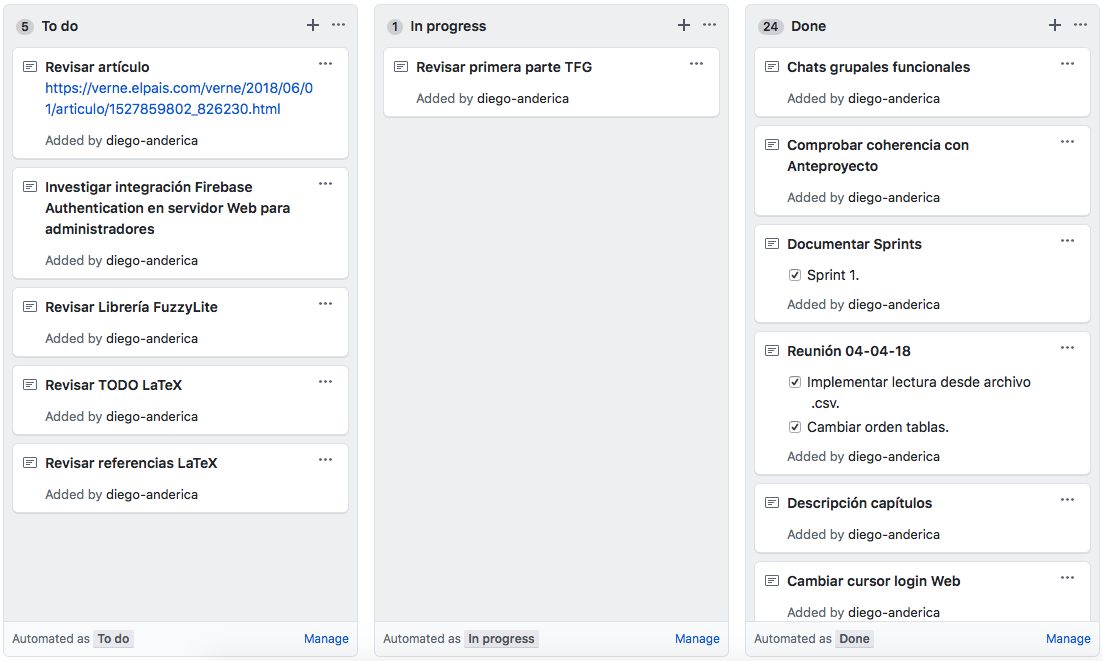
\includegraphics[width=0.75\textwidth]{/captura_kanban.png}
		\caption{Tablero Kanban en GitHub}
		\label{fig:kanban}
	\end{center}
\end{figure}

\subsubsection*{Android Studio}
Android Studio \cite{AndroidStudio} es el entorno de programación oficial para el desarrollo de aplicaciones en Android, proporcionando las herramientas necesarias para ello. Además, posee integración con Firebase, lo que permite conectar las aplicaciones con este servicio para agregar \textit{Analytics}, \textit{Authentication} y \textit{Notifications}, entre otros servicios, que resultarán imprescindibles para el desarrollo de este trabajo.

\subsubsection*{Firebase}
Firebase \cite{GooFirebase} es, principalmente, un \textit{backend} que facilita las tareas de programación en el lado del servidor, puesto que proporciona acceso fácil a los recursos que ofrece. No solo ofrece soporte al desarrollo de aplicaciones en Android, sino que también está disponible para su integración en iOS y aplicaciones web. Algunas de sus funciones son:

\begin{itemize}
	\item \textbf{\textit{Cloud Firestore}}. Se trata de una base de datos en tiempo real, siendo la evolución de \textit{Realtime Database}, ofreciendo una base de datos no relacional.
	\item \textbf{\textit{Authentication}}. Permite autenticar usuarios de forma simple en las aplicaciones de un proyecto. Además del usual método de entrada usando correo y contraseña, permite la autenticación mediante redes sociales y/o número de teléfono.
	\item \textbf{\textit{Remote Config}}. Permite modificar la aplicación de manera remota en todos los clientes sin necesidad de implementar una nueva versión.
\end{itemize}

\clearpage

Este servicio posee tres maneras de tarificación:

\begin{itemize}
	\item \textbf{Plan Spark}. Este es el plan más sencillo, con un coste gratuito. Posee ciertas limitaciones, aunque sería suficiente para un centro con un número de usuarios pequeño/medio ya que dichas limitaciones no son muy restrictivas.
	\item \textbf{Plan Flame}. Este plan tiene un coste de 25\$ (unos 21\euro{}), con lo que se eliminan las restricciones del plan básico y sería apropiado para un centro con un número de usuarios relativamente grande.
	\item \textbf{Plan Blaze}. El último plan no tiene un precio definido puesto que se paga por lo que se vaya a utilizar, por lo que es el más flexible de los tres mencionados.
\end{itemize}

\subsubsection*{IBM Bluemix}
IBM Bluemix es una plataforma que permite el acceso a sus utilidades \textit{cloud} de manera sencilla. Ofrece diversos servicios entre los que se encuentra IBM Watson. Este servicio proporciona tecnologías cognitivas para crear aplicaciones inteligentes aportando la posibilidad de analizar y comprender sentimientos o palabras claves a partir de un texto. A la hora de categorizar la adecuación de un mensaje en relación al contexto educativo se utilizará el módulo \textit{Tone Analyzer} \cite{IBM}. Al igual que sucede con Firebase, IBM Bluemix posee diferentes planes que dependen de los módulos utilizados.

\subsubsection*{LaTeX}
En cuanto a la documentación, se ha usado el lenguaje de generación de documentos LaTeX, junto con la clase \esitfg{} proporcionada \cite{ARCO}. LaTeX es un sistema de preparación de documentos de alta calidad tipográfica usado principalmente en documentos técnicos o científicos y permite a los autores centrarse más en el contenido \cite{TheLatexProject}.